\documentclass{article}

\usepackage[title]{appendix}
\usepackage{bera} % not sure I love this font for this document
\usepackage{cite}
\usepackage[letterpaper,top=2cm,bottom=2cm,left=3cm,right=3cm,marginparwidth=1.75cm]{geometry}
\usepackage{graphicx}
\usepackage[colorlinks=true, allcolors=blue]{hyperref}
\usepackage{listings}
\usepackage{wrapfig}
\usepackage{xcolor}

\colorlet{punct}{red!60!black}
\definecolor{background}{HTML}{EEEEEE}
\definecolor{delim}{RGB}{20,105,176}
\colorlet{numb}{magenta!60!black}

\lstdefinelanguage{json}{
    basicstyle=\normalfont\ttfamily,
    numbers=left,
    numberstyle=\scriptsize,
    stepnumber=1,
    numbersep=8pt,
    showstringspaces=false,
    breaklines=true,
    frame=lines,
    backgroundcolor=\color{background},
    literate=
     *{0}{{{\color{numb}0}}}{1}
      {1}{{{\color{numb}1}}}{1}
      {2}{{{\color{numb}2}}}{1}
      {3}{{{\color{numb}3}}}{1}
      {4}{{{\color{numb}4}}}{1}
      {5}{{{\color{numb}5}}}{1}
      {6}{{{\color{numb}6}}}{1}
      {7}{{{\color{numb}7}}}{1}
      {8}{{{\color{numb}8}}}{1}
      {9}{{{\color{numb}9}}}{1}
      {:}{{{\color{punct}{:}}}}{1}
      {,}{{{\color{punct}{,}}}}{1}
      {\{}{{{\color{delim}{\{}}}}{1}
      {\}}{{{\color{delim}{\}}}}}{1}
      {[}{{{\color{delim}{[}}}}{1}
      {]}{{{\color{delim}{]}}}}{1},
}

\graphicspath{ {./images/} }

\title{Developing a Visual Studio Code Language Support Extension for the Snail Programming Language}
\author{Charles Reinhardt}

\begin{document}
\maketitle

\begin{abstract}

    A high quality programming environment (often an integrated development environment, or IDE) can be vital to enhancing developer productivity. Visual Studio Code (VS Code) is a popular, open-source text editor maintained by Microsoft. VS Code delivers language-specific features through freely dowloadable, community-built extensions on an online marketplace. Many of these extensions allow developers to take advantage of editing features such as syntax highlighting, code-autocompletion, or debugging support. The snail language (Strings Numbers Arrays and Inheritance Language) is a simple, object-oriented programming langauge meant to be implemented in a one-semester undergraduate course. We present a new VS Code extension to provide language support for the snail language. The extension implements support for syntax highlighting, rudimentary auto-completion, and static error-checking diagnostics using VS Code's Langauge Server Protocol. This report summarizes the contents of a VS Code extension and gives an overview of how an extension runs, particularly highlighting the functions of VS Code's Langauge Server Protocol. I also discuss how this extension can be futher developed to make use of VS Code's Debug Adapter Protocol to implement a debugger with breakpoints, start/stop behavior, and variable inspection.

\end{abstract}

\section{Introduction}

Much of software development in the present day takes place in integrated development environments (IDEs) \cite{JetBrains_2019}. An IDE is a collection of software development tools, such as a code editor, debugger, and build system, often unified under a similar user interface, with te goal of simplifying the software development process and enhancing developer productivity \cite{Gillis_Silverthorne_2018,Shyniaieva_2023}. In addition to composing these tools together, many IDEs also offer advanced features within their code editors such as syntax highlighting, code auto-completion, and error-checking diagnostics. Today, there are any number of different IDEs available for use with any given programming language, many offered as freely-downloadable for public use. For example, a developer looking to write code in Java may choose to do so in Eclipse, IntelliJ IDEA, or BlueJ \cite{EclipseFoundation_2023, JetBrains_2023,KingsProgrammingEducationToolsGroup_2022}. With so many high quality IDEs available today, it is no surprise that 75\% of software developers today use an IDE in their everyday work \cite{JetBrains_2019}. Clearly, the IDE has become an integral part of the software development process today \cite{Vaniukov_2023}. 

Visual Studio Code (VS Code), is a popular, open source text editor maintained by Microsoft \cite{StackOverflow_2022,Microsoft_2023a}. When first downloaded, VS Code is a lightweight text editor with minimal features. However, a number of community-built, freely downloadable extensions offer advanced langauge features. These extensions can be dowloaded on VS Code's online extension marketplace, and can turn VS Code into a very fast ,robust, and powerful development environment for any programming task or language \cite{Microsoft_2023b}. 

The snail programming language (Strings Numbers Arrays and Inheritance Language) is a simple, object-oriented programming language meant to be implemented in a one-semester undergraduate course \cite{Angstadt_2023a}. In order to be implemented in a short time frame, snail is defined by limited features and a relatively annoying syntax. The language lacks a for-loop structure, opting instead to provide only while-loops. Each if statment \emph{requires} an else clause, even when the developer does not need to use one. Every statement must end with a semi-colon, which is not an issue until you accidentally forget one, and the resulting parse error message is wildly uninformative. While this design makes snail easier to implement, it makes it hard for a developer to write programs in snail.

Currently, there are no tools to offer advanced langauge support for the snail language. This is no surprise, as snail has a small user base and was first released in February 2022 \cite{Angstadt_2023b}. With no external support for the language, software developers are taken out of their comfort zone and are offered no guidance when navigating the snail language.

This report presents the Snail Language Support VS Code extension, which seeks to address the lack of programming support tools for the snail programming language. Snail Langauge Support provides several important features to make programming in the snail language easier. First, it features syntax highlighting to make reading snail code easier and help highlight key structures or keywords of the language. Further, it features rudimentary auto completion with auto-closing brackets, braces, and quotes, as well as if-else, while loop, and class definition snippets, reducing the burden of memorizing snail's strict and unintuitive syntax. The extension also has automatic, real-time error checking diagnostics that allow a user to see syntax or parse errors in a snail program before running it for themselves. Finally, the extension is structured to support a full debugger with breakpoints, step-in, step-over, and step-out functionality. 

This paper will outline the process of building the Snail Language Support VS Code extension. Specificaly, we will introduce the structure of a VS Code extension that is meant to add support for new programming langauges. We will also discuss how this extension uses VS Code's language server protocol (LSP) to provide realtime error diagnostics \cite{Microsoft_2022a}. We will address how the Snail Language Support extension may be further developed to include debugging support with breakpoints, step in/out behavior, and variable inspection, particularly highlighting the rolw of VS Code's debug adapter protocol DAP \cite{Microsoft_2021}. Finally, we will review good software development practices such as version control and documentation. 

\section{Background}

In this section, we will discuss the history of integrated development environments (IDEs) and debuggers, and how they both assist software developers today. We will also discuss Visual Studio Code (VS Code) in more detail, identifying the technologies that power VS Code. 

\subsection{History of the Modern Integrated Development Environment}

The first programming environment to remotely resemble a modern IDE was the Dartmouth BASIC programming language run on the Dartmouth Time Sharing System (DTSS), developed in the mid 1960s \cite{KemenyKurtz_1968, Kurtz_1978}. Dartmouth BASIC was an example of a compile and go system, where program compilation was not separated from program execution \cite{Weik_2001}. Additionally, the DTSS also placed focus on making sharing time on a single university computer a simpler task, in order to help make programming more accessible to novices. This makes the DTSS an early example of combining multiple software development tasks into a single programming environment.

Borland's TurboPascal takes this idea one step further. Released in 1983, TurboPascal featured a Pascal compiler, code editor, file navigation user interface, and a rudimentary debugger \cite{Gajic_2017, Intersimone_2010, Wadlow_1984}. This time period would also see language-specific IDEs in Microsoft's Visual BASIC 1.0, Microsoft's QuickC, and Borland's Turbo C/C++, all featuring similar characteristics of early IDEs \cite{Burgwin_2013, Plant_Murrell_2007, Posch_2023, Forer_Petreley_1991}.

While early IDEs certainly had their merits, they usually only supported one programming language. Microsoft's Visual Studio, released in 1997, was one of the first IDEs to package support for a variety of programming languages in one piece of software \cite{Microsoft_1997}. Visual Studio also featured extensive tools to aid in development for software on the early internet. 
T
oday, we see a trend towards open source IDEs such as Eclipse, NetBeans, or VS Code \cite{Apache_2023, EclipseFoundation_2023, Microsoft_2023a}. Even open source editors such as these include advanced development features such as an intelligent code editor, debugging tools, and version control integration. Many of these editors have advanced features within their code editors, providing functions such syntax highlighting, code autocompletion, and realtime error diagnostics. 

There are many benefits to developing software using modern IDEs. By bundling code editing, build systems, and program execution into one tool, modern IDEs reduce the time and effort a developer needs to put forth in order to test a piece of code \cite{Gillis_Silverthorne_2018}. This also reduces the number of decisions a developer has to make while developing code, which can help increase productivity. Using an IDE can also standardize the software development process, by either helping a group of people use a consistent UI (and know how to help eachother), or allow a developer to avoid switching applications to complete a single task \cite{Veracode_2020}. 

\subsection{History of Modern Debugging Tools}

Debugging is the process of searching for and fixing unexpected errors in a piece of code \cite{AWS_2023}. Early techniques of debugging software involved physically printing machine output and reading, step-by-step, through code and output, searching for a potential error \cite{RevDeBug_2020}. Some computer systems, such as the IBM 704 Data Processing system released in 2968, allowed programmers to print information stored in specified memory locations in specified forms to assist with debugging activities \cite{MIT_1957, IBMArchives_2023}. 

The \lstinline{adb} and \lstinline{dbx} debuggers for the Unix operating system saw a release in the 1970s and 1980s \cite{BellLaboratories_1983, Linton_1990}. These tols introduced the concept of breakpoints, which help a developer pinpoint the location of a fault in a piece of code. Both \lstinline{adb} and \lstinline{dbx} were run on the command line. Next, came the GNU project debugger (\lstinline{gdb}), another command line debugger, released in 1986, which gave the user even greater control of tracing a program's execution throughout its runtime \cite{GNU_FSF_2023}. With the ability to debug low-level languages like C and Assembly, \lstinline{gdb} is still in use today.

Modern debuggers with graphical user interfaces (GUIs) include the Visual Studio Debugger, which allows a developer to track variable values, function calls, and even change pieces of code or values of expressions while debugging \cite{Microsoft_2022b}. Eclipse, a popular IDE for Java, has a similar debugger with a user friendly GUI \cite{Sinha_2017}. Today, many developement workflows include the use of debugging tools \cite{Matloff_Salzman_2008}.

Debugging tools can be of great assistance to developers. By allowing developers to more closely and quickly inspect a program's execution, debugging tools can reduce the amount of time a developer spends debugging, and thus enhance developer productivity \cite{ZhRaAmRuWo_2008}. 

\subsection{What is Visual Studio Code?}

Visual Studio Code is a popular, open source code editor. Visual Studio Code is designed to be fast and lightweight, with a focus on allowing a developer to write, test, adn debug source code quickly \cite{Microsoft_2023c}. To achieve this, VS Code uses native, web, and language-specific technologoies. Tools like Electron allow VS Code to run on multiple platforms and operating systems using common web technologies like JavaScript, HTML, and CSS \cite{Electron_2023}.

While VS Code is lightweight and fast, it still supports advanced features such as build or debugger tools available through the online VS Code extension marketplace \cite{Microsoft_2023b}. VS Code is designed for extensibility, providing robust APIs to allow independent developers to create and publish extensions \cite{Microsoft_2023d}. As a result, VS Code is able to grow and develop along with its community of users. 

Existing extensions make VS Code a popular code editor \cite{StackOverflow_2022}. The CodeSnap extension allows a user to capture and share improved screenshots of code \cite{adpyke_2021}. GitLens adds additional visualization tools to help developers contribute to Git repositories while editing in VS Code \cite{GitKraken_2023}. Language Support for Java(TM) provides intellisense, formatting, refactoring, and build system support for the Java language \cite{RedHat_2023}. The result of this extension support is an IDE that is used by over 75\% of professional and hobby software developers \cite{StackOverflow_2022}. 

\section{Anatomy of a Visual Studio Code Extension}

TODO add signposting

\subsection{Directory Structure}

Most VS Code extensions share a similar directory structure. These structures may vary depending on what purpose the extension is meant to serve. In figure ~\ref{fig:directory-structure}, we see a diagram of a typical language support VS Code extension. First, the \lstinline{.vscode} directory configures how we run and test our exstension locally. Through the \lstinline{launch.json} and \lstinline{tasks.json} files, we define various tasks and configurations to streamline the build and testing process.\footnote{From personal experience, we strongly recommend taking the time to understand these files before diving into developing a VS Code extension. It will likely save painstaking debugging in the near future. See launch configurations: \url{https://code.visualstudio.com/docs/editor/debugging\#_launch-configurations} and tasks: \url{https://code.visualstudio.com/docs/editor/tasks}} It is important to note that these configuration files do not get packaged with a released VS Code extension. Next, a \lstinline{README.md} file that allows us to advertise the features of our extension. This file is rendered in the VS Code extension marketplace. We also have a \lstinline{tsconfig.json} file, which defines our TypeScript code gets transpiled to JavaScript, a topic we will discuss in further detail later in this paper. 

\begin{wrapfigure}{c}{0.3\textwidth}
    \begin{center}
        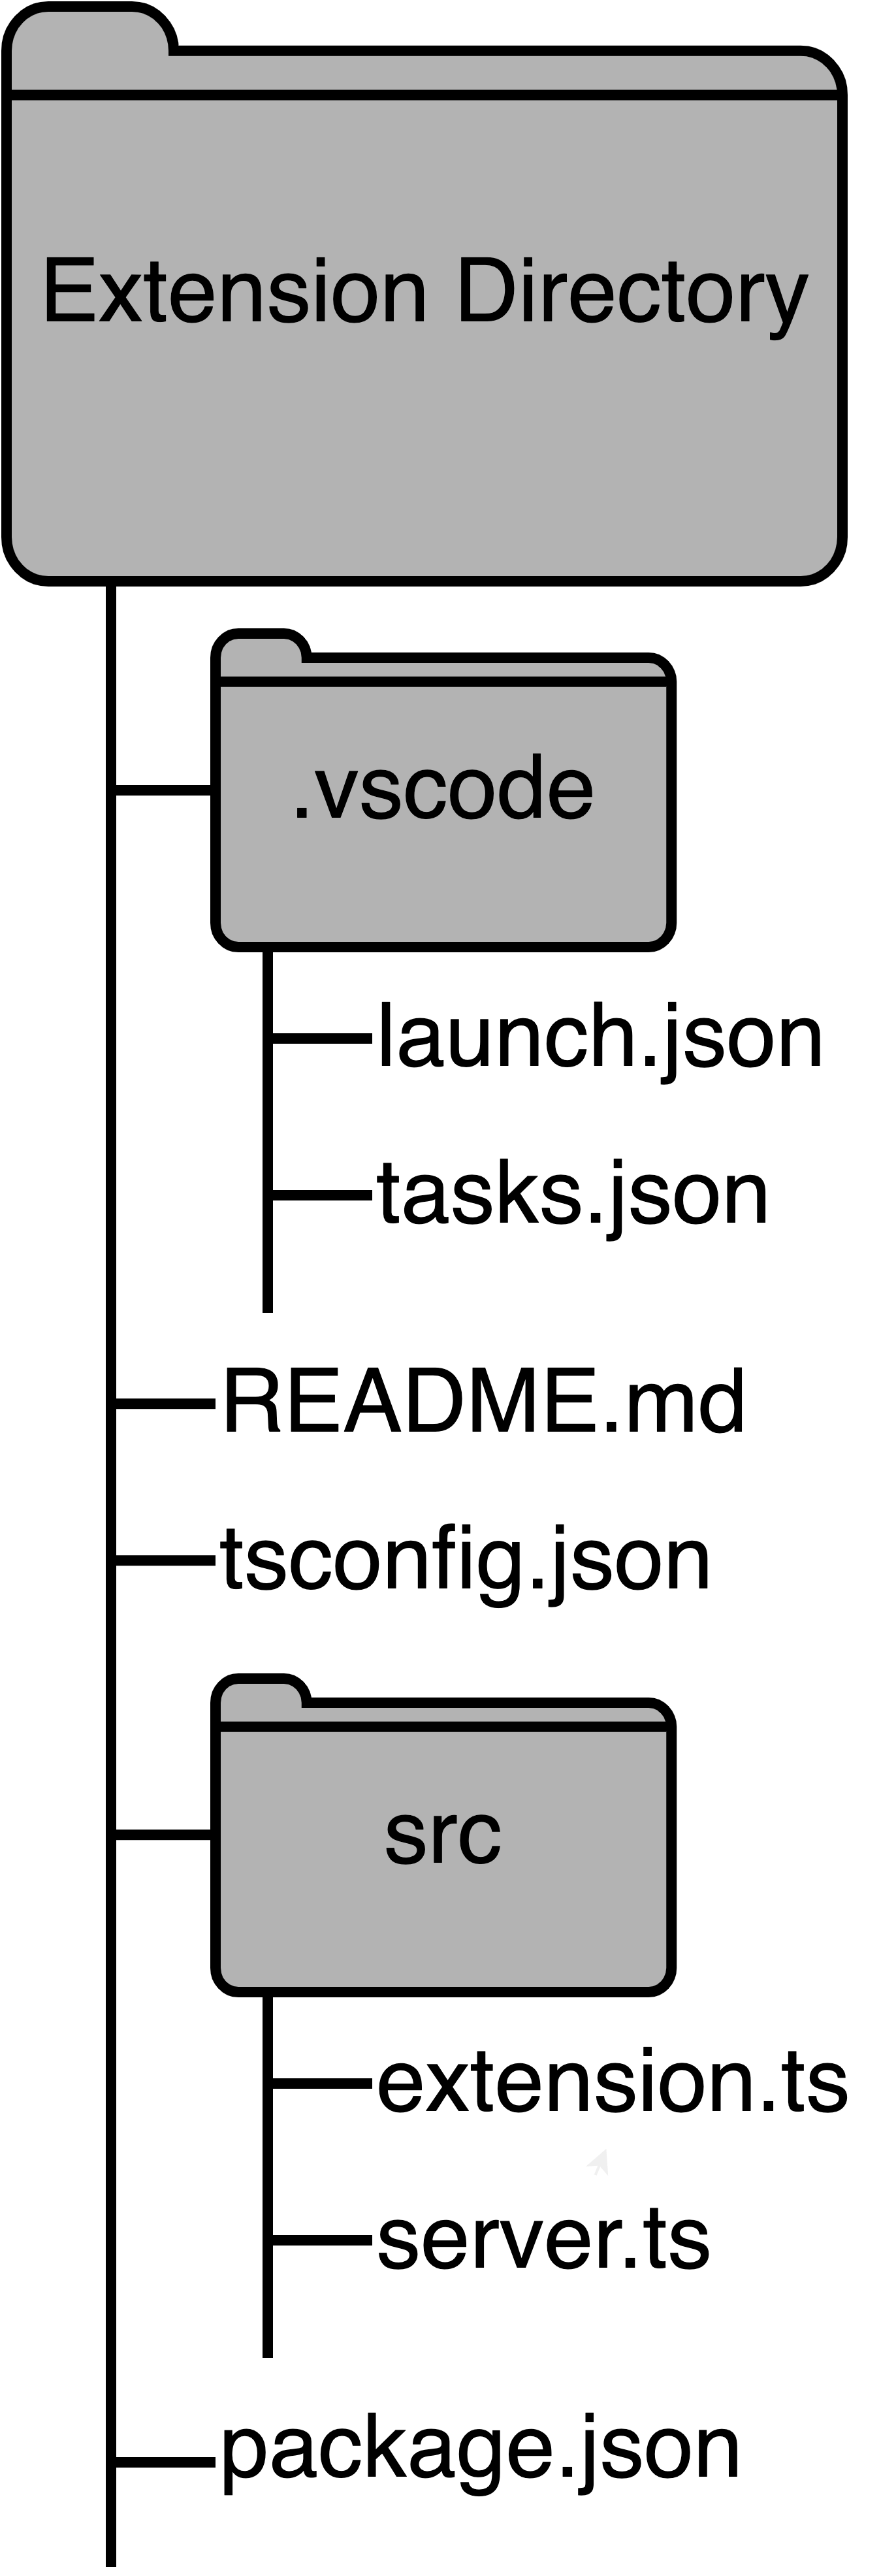
\includegraphics[height=0.3\textheight]{directory-structure.png}
        \caption{The typical directory structure of a VSCode language support extension}
    \end{center}
    \label{fig:directory-structure}
\end{wrapfigure}

The \lstinline{src} directory contains the source code that runs our extension. In this directory, the \lstinline{extension.ts} file defines special actions for our extension and launches the extension within an existing VS Code window. The \lstinline{server.ts} file defines a language server that allows our extension to take advantage of realtime error diagnostics. We further discuss language servers later in this paper. 

Lastly, the \lstinline{package.json} file defines which features and configurations our extension supports. It also contains some biographical information about the extension, such as the author, publisher, or name of the exstension. 

To build the structure for Snail Language Support, we used the \lstinline{Yeoman} tool to generate an extension skeleton \cite{Yeoman_2023}. This skeleton included configuration and source files for us to modify and build Snail Language Support on. 

We build Snail Langauge Support with TypeScript. TypeScript is a syntactic superset of JavaScript that allows the developer the benefits of a type system without sacrificing JavaScript's flexibility \cite{TypeScript_2023}. Using the TypeScript compiler (\lstinline{tsc}), a program in TypeScript is transpiled to an equivalent JavaScript program. With a \lstinline{tsconfig.json} file, we can define how the TypeScript compiler handles our TypeScript code. We define where the compiler looks for our \lstinline{.ts} files, where to place resulting JavaScript files, and the strictness of type checks during transpilation.

\subsection{Extension Contributions: The Extension Manifest}

Recall that the \lstinline{package.json} defines what our extension contributes to the user. We now dive into what some of those contributions might be.

First, we can define some metadata about our extension, such as a name, author, description, and version. We can also define which version of the VS Code engine this extension expects. This ensures that an extension knows which VS Code APIs it has proper access to. For example, an extension that expects a VS Code version of \lstinline{1.7.0} won't be able to take advantage of an API released in \lstinline{1.8.0} \cite{Microsoft_2023e}. We can also define some categories that our extension falls under, helping our extension gain visibility on the online VS Code marketplace.

Next, and very importantly, we can define activations events that define when our extension becomes active. When VS Code detects a given activation event, it calls the \lstinline{activate} function found in our \lstinline{extension.ts} file. For example, \lstinline{onLanguage:snail} says that Snail Language Support should be activated when a user is viewing a snail language file. We also define where VS Code looks for the \lstinline{activate} function with our \lstinline{main} attribute. For a more detailed look at Snail Language Support's \lstinline{package.json} file, see Appendix \ref{app:package-json}.

\subsection{Extension Lifecycle: From Startup to Shutdown}

Here, we discuss what happens under the hood when VS Code runs an extension.

When a VS Code client detects an extension's defined activation events, it reads the \lstinline{main} attribute of \lstinline{package.json} to call the \lstinline{activate} function defined in that file. This file (in Snail Language Support's case, the \lstinline{extension.ts} file) has access to the VS Code extension API, which allows us to update the VS Code client UI \cite{Microsoft_2023d}. For example, depending on a user's configuration settings, Snail Language Support can display a VS Code UI style error message window to the user.  
    
Also in this file, we register a few command handlers to watch for commands input from a user. These command handlers are examples of the observer design pattern, which allow a developer to handle a variety of input events that are experienced during runtime \cite{GangOfFour_1995}. A developer can register an observer that waits and listens for a particular event, and executes a block of code once that event is detected. One of these command handlers responds to snail file debugging requests. We will touch on the topic of debugging within Snail Language Support more later. 

We also launch our language server, which communicates via VS Code's Language Server Protocol (LSP), inside of our \lstinline{activate} function. We further discuss this topic later.

\subsection{Language Configuration}

\subsection{Rudimentary Autocompletion Through Snippets}

\subsection{Syntax Highlighting}

\section{Language Servers and the Language Server Protocol (LSP)}

\subsection{Theory}

\subsection{LSP in Snail Language Support}

\section{Debug Adapter Protocol}

\subsection{Theory}

\subsection{Debug Adapter Protocol in Snail Language Support}

\section{Good Practices in Software Development}

\subsection{Version Control}

\subsection{Documentation}

\section{Conclusions}

%== BIBLIOGRAPHY ==%
\newpage

\bibliography{refs.bib}
\bibliographystyle{plain}

%== APPENDICES ==%
\newpage

\begin{appendices}

\section{Snail Language Support package.json}

    The following is the \lstinline{package.json} file from Snail Language Support.
    \lstinputlisting[language=json]{
        % this absolute path must be different when building on different machines
        /Users/charlesreinhardt/Git/snail-language-support/package.json
    }
    \label{app:package-json}

\end{appendices}

\end{document}